
\documentclass[12pt,oneside,a4paper]{article}

\usepackage{float}
%\floatstyle{boxed}
%\restylefloat{figure}

\usepackage{tabularx}
\usepackage{multirow}

\usepackage[svgnames,table]{xcolor}


\def\dustRowHead{LightSlateGrey}
\def\dustRowFirst{LightGray}
\def\dustRowSecond{White}

%\rowcolor{\dustRowSecond}
%\rowcolors{1}{\dustRowFirst}{\dustRowSecond}

\usepackage{amsmath}
\usepackage{amsfonts}
\usepackage{amssymb}

\usepackage{wallpaper}

\usepackage{tikz}
\usepackage{tkz-euclide}

\usepackage{pgfplots}

\usepackage[section]{placeins}

\usepackage[
    top=2.5cm,
    bottom=2.5cm,
    left=4cm,
    right=2.5cm
]{geometry}

\ifdefined\DEBUG
    \usepackage{showframe}
\fi

\usepackage[gen]{eurosym}

%\renewcommand{\familydefault}{\sfdefault}
\usepackage[utf8]{inputenc}

\usepackage[english]{babel}
\usepackage{csquotes}

\usepackage{graphicx}

\usepackage[round]{natbib}

\usepackage{setspace}
\onehalfspacing

\usepackage[ddmmyyyy]{datetime}
\renewcommand{\dateseparator}{.}
%\newdate{date}{06}{07}{2015}
%\date{\displaydate{date}}

\ifdefined\PRINT
    \usepackage[hidelinks]{hyperref}
\else
    \usepackage{hyperref}
\fi

\usepackage[xindy]{glossaries}


\newglossaryentry{python}{
    name=Python,
    description={
        A widely used scripting language with focus on readable source-code.
    }
}

\newglossaryentry{pybottle}{
    name=bottle,
    description={
        A python based web-framework that supports routing, templates and contains a web-server.
    }
}

\newglossaryentry{sqlite}{
    name=SQLite,
    description={
        A relational database system with support of Transactions and Views. It is also included in one of the standard Python-modules.
    }
}

\newglossaryentry{sphinx}{
    name=Sphinx,
    description={
        A document generator initially built for Python. It creates a documentation from docstrings within the Python source code.
    }
}










\usepackage{listingsutf8}
\lstset{
    belowcaptionskip=1\baselineskip,
    breaklines=true,
    frame=L,
    xleftmargin=\parindent,
    language=HTML,
    showstringspaces=false,
    basicstyle=\footnotesize\ttfamily,
    keywordstyle=\bfseries\color{green!40!black},
    commentstyle=\itshape\color{purple!40!black},
    identifierstyle=\color{blue},
    stringstyle=\color{orange},
    numbers=left,
    numberstyle=\tiny,
    escapeinside={°(}{)°},
}


\begin{document}

% titlepage


\newcommand{\TitleHRule}{\rule{\linewidth}{0.5mm}}

\begin{titlepage}

    \begin{center}

    { \huge \bfseries Clothing recommendation based on rocchio's algorithm\\[0.4cm]}
    { \huge -\\[0.4cm]}
    { \huge Design and prototypical implementation}
    
    \TitleHRule
    \bigskip

    \includegraphics[width=70mm]{./inc/title/fau-logo}
    \bigskip

    Zwischenbericht zur Erlangung des akademischen Grades\\
    Bachelor of Science\\
    an der Friedrich-Alexander Universit\"at Erlangen-N\"urnberg\\

    \TitleHRule

    \begin{tabular}{ l l }
        Eingereicht von:    & Dusty Wind\\
                            & Strasse Hausnummer\\
                            & PLZ Wohnort\\
        Matrikelnummer:     & Matrikelnummer\\
        Studiengang         & Studiengang\\
        Referent            & Prof. Dr. Freimut Bodendorf\\
        Betreuer            & Betreuer
    \end{tabular}

    \TitleHRule
    


    \end{center}

\end{titlepage}








% Table of content
\tableofcontents
\clearpage

% the text

\section{Introduction}
\iffalse
{\color{red} 
TODO:
\begin{itemize}
    \item item == document
    \item web-api
    \item doc-comments in source code
    \imte use case
\end{itemize}
}
\fi

%\subsection{Motivation}
% Choice overload
% Aktuelle Situation in der Kleidungsbranche
% kurzer Einblick in Recommender systems (wird spaeter weiter ausgefuehrt)
\noindent
When a typical customer enters a shop or department store, he often gets confronted with a very huge collection of products he can choose from.
This is especially true, when searching for products online on a web shop.
The commonly well-known web shop \gls{amazon.com}, for instance, provides about 280 million different products on their internet presence solely for the United States - there are even more products offered world wide.\citep{marketplaceanalytics:2014}
Even shops dedicated to only a special kind of product can have a wide array of products.
On \gls{zalando}, a German online shop dedicated to clothing, one can choose out of 150.000 products and 1.500 different brands.\citep{visser:2014}

%\paragraph{Choice Overload}
\index{Choice Overload}
There is a general belief that great choice pleases the customer's needs.
However it is actually proven that this idea is not fully correct and reality is much more complex.
Already in 2000 a group of scientists demonstrated that a great variety can also have negative effects.
It is proven that large assortments can lower the customer's willingness to purchase products.\citep[p.~312-313]{diehl:2010}
Furthermore, too much choice can also lower the customer's satisfaction.\citep[p.~320]{diehl:2010}
The state of being confronted with an overwhelming range of choice and therefore having trouble finding the right product is commonly known as choice overload.\citep[p.~454]{stanton:2012}
Even though huge assortment of products attract user, because they generally like to have the possibility to choose, it increases the psychological costs to filter out relevant products and make a decision.
In the end the whole benefit the user may get from a huge assortment of products gets fully consumed by the energy he has to spend in order to find a good that meets his expectations.
\citep[p.~64]{bollen:2010}

\index{Recommender System}
One possible solution to solve problems caused by choice overload are recommender systems (RS) as they help users finding relevant items they like, by guiding them to those items in a huge space of products.\citep[p.~63]{bollen:2010}
Since especially online-shops have an overwhelming assortment of products, they struggle most with the problem of overloading their potential customers with choice.
Therefore many \gls{e-commerce} sites have already implemented recommendation systems to aid their customers in finding the best product.
Popular e-commerce sites such as Amazon.com and \gls{eBay} rely heavily on RS in order to satisfy their customers needs.
In fact some vendors even use multiple RS for different use cases to maximise the support they can provide to customers.
\citep[p.~158]{schafer:1999}
There are different possible approaches to recommender systems and some of them will be discussed in the later sections (section~\ref{sec:recommenderapproaches}) of this thesis.
This thesis, however, focuses on implementing a recommender system, all necessary steps towards the implementation and finally an evaluation of its aptitude.
As algorithm for the recommender engine Rocchio's algorithm will be implemented.
There will also be an evaluation about different ways of collecting information from the user.


\subsection{Research question}
This thesis aims for designing and implementing a recommender system based on Rocchio's algorithm.
In order to reach this goal it is necessary to specify the overall benefit a RS can offer and all tasks it has to solve.
This knowledge will be used to define requirements to a recommender system.
These requirements are necessary for implementing a RS.
Also the built recommender system will be used as basis for an abstract online-shop to visualize the interaction and results.
When designing a recommendation system there are a couple of questions, such as its requirements, left to answer.

These research questions will be defined first.
%In the following all requirements on a recommender system will be defined.
%\\
The remaining thesis will orient its basic structure on the research questions.

At first the general fundamentals of RS will be explained.
Since a major goal of this thesis is the implementation of an RS it is necessary to identify the core components of which a RS is build of and the tasks it has to solve.

Followed up by a state of the art analysis where the current situation and possible approaches for RS will be discussed.
There are many approaches for generating automated recommendations such as ``content-based", ``collaborative filtering", ``demographic", ``knowledge-based", ``community-based".\citep[p.~10-12]{ricci:2011}
In addition there are various forms of user feedback which can vary from implicit to explicit.\citep[p.~76]{lops:2011}
Since there are so many possibilities it is important to identify those approaches which are best suited for recommending clothing and to categorize Rocchio's algorithm.

When basic knowledge about RS has been built up all prerequisites for Rocchio's algorithm, such as the question how the computer representation can be implemented, will be satisfied.
It will also be evaluated to which extend the algorithm can be adjusted at runtime in order to react at some event (for example when the user of the RS changes his mind about a certain kind of product).
Rocchio's algorithm on its own can only give a representation of the users wishes.
To identify recommendations based on the users ideas there are some more components necessary which remain left to find.

When the major goal of implementing a RS based on Rocchio's algorithm has been achieved, its results will be examined.
With this the main question of how good the recommendations of a RS based on Rocchio's algorithm will be can be solved.

In the end there are some suggestions on how to use Rocchio's algorithm in a real application - either in the ``real world", or on an online shop.

The research questions derived from this paragraph are summarized in figure~\ref{fig:research-questions}.


\begin{figure}[h!]
    \center
    \begin{tikzpicture}
        %\def\dustTempLineWidth{12cm}
        \def\dustTempLineWidth{10cm}
        \def\dustTempNodeWidth{4cm}
        %\def\dustTempNodeHeight{4cm}
        \def\dustTempNodeHeight{3cm}
        \def\dustTempArrowHeight{1cm}
        \def\dustTempYShift{0cm}
        \def\dustTempLineColour{Black!20}

        \def\dustTempEnumerateLabel{\bfseries Q\arabic* :}

        \def\dustTempYShift{0 * -1 * (\dustTempNodeHeight + \dustTempArrowHeight)}
        \draw[thick,fill=\dustRowFirst]
            (0,0)--(\dustTempNodeWidth /2,-1* \dustTempArrowHeight)--(\dustTempNodeWidth,0)--(\dustTempNodeWidth,\dustTempNodeHeight)--(0,\dustTempNodeHeight)--cycle;
        \node[text width=\dustTempNodeWidth,text centered,yshift=\dustTempYShift] at (\dustTempNodeWidth /2,\dustTempNodeHeight /2)
        {
            \textbf{Requirements on a recommender system}
        };
        \node[text width=\dustTempLineWidth,align=left,yshift=\dustTempYShift] at ({\dustTempNodeWidth + \dustTempLineWidth /2 + 0.5cm},\dustTempNodeHeight/2) {
            \begin{enumerate}[label=\dustTempEnumerateLabel]
                \item What are the key requirements a recommender system has to fulfill?
            \end{enumerate}
        };
        \draw[thin,\dustTempLineColour,yshift=\dustTempYShift] (\dustTempNodeWidth,0)--(\dustTempNodeWidth + \dustTempLineWidth,0);

        \def\dustTempYShift{1 * -1 * (\dustTempNodeHeight + \dustTempArrowHeight)}
        \draw[thick,fill=\dustRowSecond,yshift=\dustTempYShift]
            (0,0)--(\dustTempNodeWidth /2,-1 * \dustTempArrowHeight)--(\dustTempNodeWidth,0)--(\dustTempNodeWidth,\dustTempNodeHeight+\dustTempArrowHeight)--(\dustTempNodeWidth /2,\dustTempNodeHeight)--(0,\dustTempNodeHeight + \dustTempArrowHeight)--cycle;
        \node[text width=\dustTempNodeWidth,text centered,yshift=\dustTempYShift] at (\dustTempNodeWidth /2,\dustTempNodeHeight /2)
        {
            \textbf{Different approaches}
        };
        \node[text width=\dustTempLineWidth,align=left,yshift=\dustTempYShift] at ({\dustTempNodeWidth + \dustTempLineWidth /2 + 0.5cm},\dustTempNodeHeight /2 + \dustTempArrowHeight /2)
        {
            %\begin{quote}
                %There are many approaches to generate automated recommendations. % such as "content-based", "collaborative filtering", "demographic", "knowledge-based", "community-based".\citep[p.~10-12]{ricci:2011}
                %Also the source of user feedback can vary from implicit to explicit feedback.\citep[p.~76]{lops:2011}
                %How do they work and which approach does rocchio's algorithm take?
            %\end{quote}
            \begin{enumerate}[label=\dustTempEnumerateLabel]
                \setcounter{enumi}{1}
                \item Which of these approaches is best suited to generate clothing-recommendations based on implicit feedback?
            \end{enumerate}
        };
        \draw[thin,\dustTempLineColour,yshift=\dustTempYShift] (\dustTempNodeWidth,0)--(\dustTempNodeWidth + \dustTempLineWidth,0);

        \def\dustTempYShift{2 * -1 * (\dustTempNodeHeight + \dustTempArrowHeight)}
        \draw[thick,fill=\dustRowFirst,yshift=\dustTempYShift]
        (0,0)--(\dustTempNodeWidth /2,-1 * \dustTempArrowHeight)--(\dustTempNodeWidth,0)--(\dustTempNodeWidth,\dustTempNodeHeight+\dustTempArrowHeight)--(\dustTempNodeWidth /2,\dustTempNodeHeight)--(0,\dustTempNodeHeight + \dustTempArrowHeight)--cycle;
        \node[text width=\dustTempNodeWidth,text centered,yshift=\dustTempYShift] at (\dustTempNodeWidth /2,\dustTempNodeHeight /2)
        {
            \textbf{Computer representation}
        };
        \node[text width=\dustTempLineWidth,align=left,yshift=\dustTempYShift] at ({\dustTempNodeWidth + \dustTempLineWidth /2 + 0.5cm},\dustTempNodeHeight /2 + \dustTempArrowHeight /2)
        {
            \begin{enumerate}[label=\dustTempEnumerateLabel]
                \setcounter{enumi}{2}
                \item How can products be represented on a computer?
                %\item Can the Rocchio algorithm be adjusted at run-time?
                \item How well can Rocchio's algorithm be adjusted at run-time?
                \item How can possible recommendations be found?
            \end{enumerate}
        };
        \draw[thin,\dustTempLineColour,yshift=\dustTempYShift] (\dustTempNodeWidth,0)--(\dustTempNodeWidth + \dustTempLineWidth,0);

        \def\dustTempYShift{3 * -1 * (\dustTempNodeHeight + \dustTempArrowHeight)}
        \draw[thick,fill=\dustRowSecond,yshift=\dustTempYShift]
        (0,0)--(\dustTempNodeWidth /2,-1 * \dustTempArrowHeight)--(\dustTempNodeWidth,0)--(\dustTempNodeWidth,\dustTempNodeHeight+\dustTempArrowHeight)--(\dustTempNodeWidth /2,\dustTempNodeHeight)--(0,\dustTempNodeHeight + \dustTempArrowHeight)--cycle;
        \node[text width=\dustTempNodeWidth,text centered,yshift=\dustTempYShift] at (\dustTempNodeWidth /2,\dustTempNodeHeight /2)
        {
            \textbf{Testing}
        };
        \node[text width=\dustTempLineWidth,align=left,yshift=\dustTempYShift] at ({\dustTempNodeWidth + \dustTempLineWidth /2 + 0.5cm},\dustTempNodeHeight /2 + \dustTempArrowHeight /2)
        {
            \begin{enumerate}[label=\dustTempEnumerateLabel]
                \setcounter{enumi}{5}
                \item Are the results of the algorithm (tested in a self-built online-shop) satisfying?
            \end{enumerate}
        };
        \draw[thin,\dustTempLineColour,yshift=\dustTempYShift] (\dustTempNodeWidth,0)--(\dustTempNodeWidth + \dustTempLineWidth,0);

        \def\dustTempYShift{4 * -1 * (\dustTempNodeHeight + \dustTempArrowHeight)}
        \draw[thick,fill=\dustRowFirst,yshift=\dustTempYShift]
            (0,0)--(\dustTempNodeWidth,0)--(\dustTempNodeWidth,\dustTempNodeHeight + \dustTempArrowHeight)--(\dustTempNodeWidth /2,\dustTempNodeHeight)--(0,\dustTempNodeHeight + \dustTempArrowHeight)--cycle;
        \node[text width=\dustTempNodeWidth,text centered,yshift=\dustTempYShift]at (\dustTempNodeWidth /2,\dustTempNodeHeight /2)
        {
            \textbf{Outlook}
        };
        \node[text width=\dustTempLineWidth,align=left,yshift=\dustTempYShift] at ({\dustTempNodeWidth + \dustTempLineWidth /2 + 0.5cm},\dustTempNodeHeight /2 + \dustTempArrowHeight /2)
        {
            \begin{enumerate}[label=\dustTempEnumerateLabel]
                \setcounter{enumi}{6}
                \item How can Rocchio's algorithm be implemented in a ``real" (online-)shop?
            \end{enumerate}
        };
        \draw[thin,\dustTempLineColour,yshift=\dustTempYShift] (\dustTempNodeWidth,0)--(\dustTempNodeWidth + \dustTempLineWidth,0);

    \end{tikzpicture}

    \caption{Overview of research questions}
    \label{fig:research-questions}

\end{figure}


%\FloatBarrier


%Wie kann ein system konzeptioniert und implementiert zu werden um efektive kleidungsempfehlung basierend auf implizitem feedback zu geben?


%- Forschungsmethodik/Vorgehen
%   -- vorgehen mit beispiel der Forschungsfragen

\subsection{Research methodology}
One of this thesis' core aspects is the implementation of a recommender system using Rocchio's algorithm.
This implementation will be combined with an online-shop.
Since a fully developed online shop would be out of scope for this thesis the implemented shop will only concentrate on the core-components necessary for generating recommendations such as presenting products and receiving feedback from the user.

A characteristic of the algorithm in use is its way of refining the set of recommendations every time a user gives more information about his preferences.\citep[p. 92]{lops:2011}
%The process of learning about the user can be both implicit, or explicit.
%Learning based on implicit behaviour will be implemented in the first version.
%Depending on the time schedule an alternative implementation with explicit user feedback is possible.\\

Because developing software is much more than solely writing source code, there will also be a proper documentation.
The source code will also be illustrated by ER- and UML-diagrams in order to make the concept easier to understand on a more abstract level than source code.

\paragraph{Proceeding}
By the time the project is finished there will be two software-components.
\\
First, a programming library (called recommender.lib) which is capable of handling product-data and generating recommendation for any user based on his recorded (shopping-)behaviour.
Second, an online shop that presents products and provides recommendations for products the user might like, based on recommender.lib.
As programming language for implementing the recommender-library Python has been chosen.
In order to make the library interoperable with other programming languages a web-API may be built.

\paragraph{Documentation}
The theory of the code will be explained in a separate document with many examples to visualize the way the recommendation system works.
Additionally there will be a documentation based on python-sphinx which will be automatically generated out of source-code comments.

\paragraph{Milestones}
The development of the recommender algorithm will be subdivided into stages.
These can be seen in figure~\ref{fig:softwaremilestones}.
Each of the steps has to be finished before the next can start.
\\

\begin{figure}[h!]
    \centering
    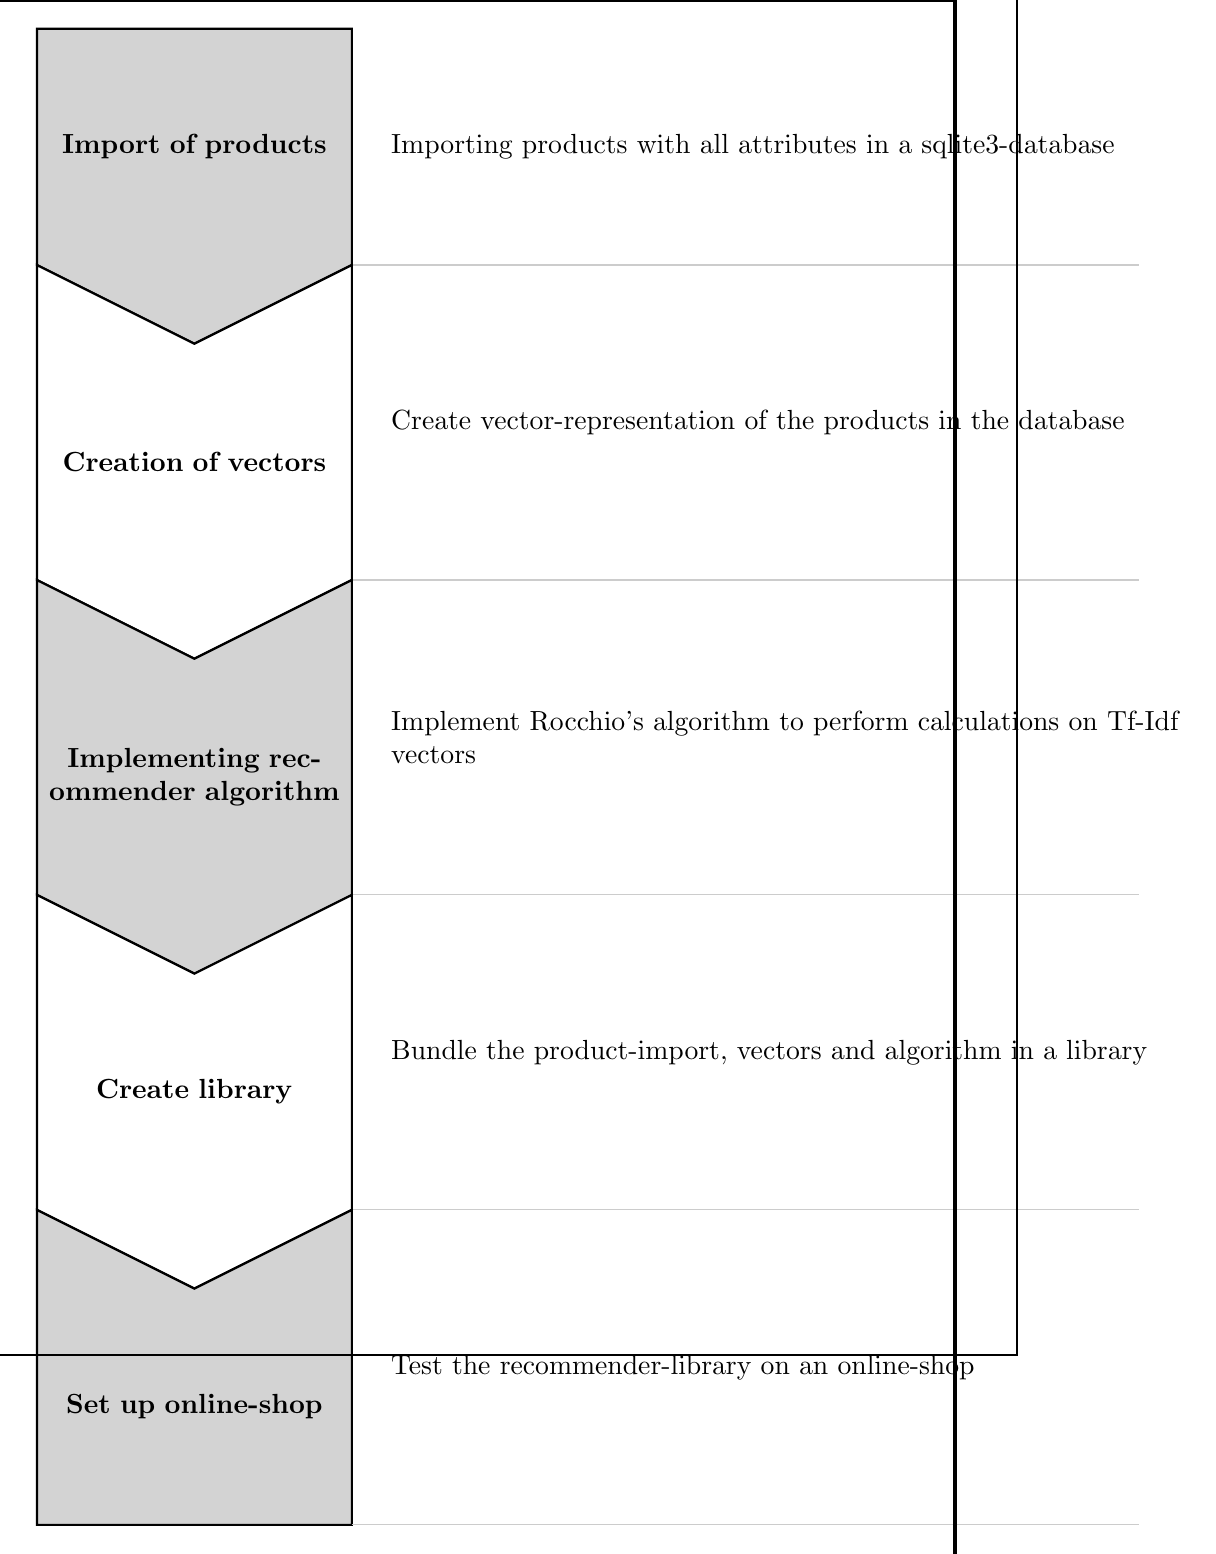
\begin{tikzpicture}
        %\def\dustTempLineWidth{12cm}
        \def\dustTempLineWidth{10cm}
        \def\dustTempNodeWidth{4cm}
        %\def\dustTempNodeHeight{4cm}
        \def\dustTempNodeHeight{3cm}
        \def\dustTempArrowHeight{1cm}
        \def\dustTempYShift{0cm}
        \def\dustTempLineColour{Black!20}

        \def\dustTempYShift{0 * -1 * (\dustTempNodeHeight + \dustTempArrowHeight)}
        \draw[thick,fill=\dustRowFirst]
            (0,0)--(\dustTempNodeWidth /2,-1* \dustTempArrowHeight)--(\dustTempNodeWidth,0)--(\dustTempNodeWidth,\dustTempNodeHeight)--(0,\dustTempNodeHeight)--cycle;
        \node[text width=\dustTempNodeWidth,text centered,yshift=\dustTempYShift] at (\dustTempNodeWidth /2,\dustTempNodeHeight /2)
        {
            \textbf{Import of products}
        };
        \node[text width=\dustTempLineWidth,align=left,yshift=\dustTempYShift] at ({\dustTempNodeWidth + \dustTempLineWidth /2 + 0.5cm},\dustTempNodeHeight/2)
        {
            Importing products with all attributes in a sqlite3-database
        };
        \draw[thin,\dustTempLineColour,yshift=\dustTempYShift] (\dustTempNodeWidth,0)--(\dustTempNodeWidth + \dustTempLineWidth,0);

        \def\dustTempYShift{1 * -1 * (\dustTempNodeHeight + \dustTempArrowHeight)}
        \draw[thick,fill=\dustRowSecond,yshift=\dustTempYShift]
            (0,0)--(\dustTempNodeWidth /2,-1 * \dustTempArrowHeight)--(\dustTempNodeWidth,0)--(\dustTempNodeWidth,\dustTempNodeHeight+\dustTempArrowHeight)--(\dustTempNodeWidth /2,\dustTempNodeHeight)--(0,\dustTempNodeHeight + \dustTempArrowHeight)--cycle;
        \node[text width=\dustTempNodeWidth,text centered,yshift=\dustTempYShift] at (\dustTempNodeWidth /2,\dustTempNodeHeight /2)
        {
            \textbf{Creation of vectors}
        };
        \node[text width=\dustTempLineWidth,align=left,yshift=\dustTempYShift] at ({\dustTempNodeWidth + \dustTempLineWidth /2 + 0.5cm},\dustTempNodeHeight /2 + \dustTempArrowHeight /2)
        {
            Create vector-representation of the products in the database
        };
        \draw[thin,\dustTempLineColour,yshift=\dustTempYShift] (\dustTempNodeWidth,0)--(\dustTempNodeWidth + \dustTempLineWidth,0);

        \def\dustTempYShift{2 * -1 * (\dustTempNodeHeight + \dustTempArrowHeight)}
        \draw[thick,fill=\dustRowFirst,yshift=\dustTempYShift]
        (0,0)--(\dustTempNodeWidth /2,-1 * \dustTempArrowHeight)--(\dustTempNodeWidth,0)--(\dustTempNodeWidth,\dustTempNodeHeight+\dustTempArrowHeight)--(\dustTempNodeWidth /2,\dustTempNodeHeight)--(0,\dustTempNodeHeight + \dustTempArrowHeight)--cycle;
        \node[text width=\dustTempNodeWidth,text centered,yshift=\dustTempYShift] at (\dustTempNodeWidth /2,\dustTempNodeHeight /2)
        {
            \textbf{Implementing recommender algorithm}
        };
        \node[text width=\dustTempLineWidth,align=left,yshift=\dustTempYShift] at ({\dustTempNodeWidth + \dustTempLineWidth /2 + 0.5cm},\dustTempNodeHeight /2 + \dustTempArrowHeight /2)
        {
            Implement Rocchio's algorithm to perform calculations on Tf-Idf vectors
        };
        \draw[thin,\dustTempLineColour,yshift=\dustTempYShift] (\dustTempNodeWidth,0)--(\dustTempNodeWidth + \dustTempLineWidth,0);

        \def\dustTempYShift{3 * -1 * (\dustTempNodeHeight + \dustTempArrowHeight)}
        \draw[thick,fill=\dustRowSecond,yshift=\dustTempYShift]
        (0,0)--(\dustTempNodeWidth /2,-1 * \dustTempArrowHeight)--(\dustTempNodeWidth,0)--(\dustTempNodeWidth,\dustTempNodeHeight+\dustTempArrowHeight)--(\dustTempNodeWidth /2,\dustTempNodeHeight)--(0,\dustTempNodeHeight + \dustTempArrowHeight)--cycle;
        \node[text width=\dustTempNodeWidth,text centered,yshift=\dustTempYShift] at (\dustTempNodeWidth /2,\dustTempNodeHeight /2)
        {
            \textbf{Create library}
        };
        \node[text width=\dustTempLineWidth,align=left,yshift=\dustTempYShift] at ({\dustTempNodeWidth + \dustTempLineWidth /2 + 0.5cm},\dustTempNodeHeight /2 + \dustTempArrowHeight /2)
        {
            Bundle the product-import, vectors and algorithm in a library
        };
        \draw[thin,\dustTempLineColour,yshift=\dustTempYShift] (\dustTempNodeWidth,0)--(\dustTempNodeWidth + \dustTempLineWidth,0);

        \def\dustTempYShift{4 * -1 * (\dustTempNodeHeight + \dustTempArrowHeight)}
        \draw[thick,fill=\dustRowFirst,yshift=\dustTempYShift]
            (0,0)--(\dustTempNodeWidth,0)--(\dustTempNodeWidth,\dustTempNodeHeight + \dustTempArrowHeight)--(\dustTempNodeWidth /2,\dustTempNodeHeight)--(0,\dustTempNodeHeight + \dustTempArrowHeight)--cycle;
        \node[text width=\dustTempNodeWidth,text centered,yshift=\dustTempYShift]at (\dustTempNodeWidth /2,\dustTempNodeHeight /2)
        {
            \textbf{Set up online-shop}
        };
        \node[text width=\dustTempLineWidth,align=left,yshift=\dustTempYShift] at ({\dustTempNodeWidth + \dustTempLineWidth /2 + 0.5cm},\dustTempNodeHeight /2 + \dustTempArrowHeight /2)
        {
            Test the recommender-library on an online-shop
        };
        \draw[thin,\dustTempLineColour,yshift=\dustTempYShift] (\dustTempNodeWidth,0)--(\dustTempNodeWidth + \dustTempLineWidth,0);

    \end{tikzpicture}

    \caption{Software milestones for building a recommender system}
    \label{fig:softwaremilestones}
\end{figure}




\section{Recommender systems in general}
\index{Recommender System}
As already mentioned RS help users fiding relevant items by filtering them out.
Depending on the context these items can be of any form.
%In a e-commerce context for example, these items can be a selection of products a online shop has.
In the context of an e-commerce site those items could be a selection of products the online shop offers.
A item in the context of a library, however, could be books which are free to borrow.
\citep[p.~377-378]{burke:2007}

%{\color{red}RS noch mal besser beschreiben (wie in der einf\"uhrung nur genauer)}
%Even though has already been a brief introduction into recommender systems a much more in depth view will follow.
When describing a RS, one also has to describe the different users and the goal they want to achieve.
On the one hand is the provider of an RS - for the time being let's assume that the provider is a huge online shop selling apparel.
On the other hand is the client using an offered RS to simplify the search for products best suited for his needs.
In case of a online shop the user's primary intention if finding clothing that is after his fancy and in his size.
The online shop however, pursues many more objectives.
When he offers a RS to the user, he wants to
\begin{itemize}
    \item\textbf{Increase sells}\hfill\\
        By determining and offering the items the user likes most, the chance of the user buying the praised product will increase.
    \item\textbf{Selling more diverse items}\hfill\\
        Often the user only has a vague idea of the product he wants and only knows the well-established ones.
        RS can help to recommend products he needs and he wouldn't have found otherwise.
    \item\textbf{Increase user satisfaction to gain customer loyalty}\hfill\\
        %{\color{red} Explain in detail.}
        With good recommendations and a pleasing user interface the user is more likely to accept recommendations.
    \item\textbf{Increase user fidelity}\hfill\\
        A RS links the users' usage behaviour to his previous one.
        %A RS links the using behaviour to the users previous one.
        This helps to get a more accurate picture of the user's preferences.
    \item\textbf{Gain better understanding about the users needs}\hfill\\
        When the general preferences of users are known, it is possible to adapt the internal work flow of the RS provider to the user.
        This means, that an apparel shop can increase the stock on some specific cuts/patterns or colours, since the customers will demand them.
\end{itemize}
as mentioned by \citeauthor{ricci:2011}.\citep[p.~4-5]{ricci:2011}
\\

In contrast to the RS provider the user has way more diverse objectives.
\citeauthor{herlocker:2004} defined the most common tasks a RS has to fulfill in order to suit the users needs.
\begin{itemize}
    \item\textbf{Annotation in context}\hfill\\
        Given a catalog of items a RS can highlight those of which it believes to be relevant to the user.
    \item\textbf{Find good items}\hfill\\
        Provide users with a list of recommended items plus an estimation of how likely the item appeals to the user.
    \item\textbf{Find all good items}\hfill\\
        In order to reduce choice overload RS filter out most of the good items which may attract the user.
        Due to the filtering it may happen that not all of the items which could please the users needs will be recommended.
        In some domains however this must not happen.
        Or to put it into search engine terminology: The recall must be as high as possible.
    \item\textbf{Recommend sequence}\hfill\\
        Instead of recommending items that fulfill all requirements on their own it is also possible to recommend a combination of items.
        Rather than a single item a composite of items will be recommended to the user.
    \item\textbf{Just browsing}\hfill\\
        It has been noticed that many user browse through website without the intention of buying items but rather looking through the assortment offered.
        In such cases a RS doesn't have to make precise recommendations, since they do not matter anyway.
    \item\textbf{Find credible recommender}\hfill\\
        Users that are aware of the fact that their search for items is supported by a recommender system tend to purposely test the recommender systems quality.
        This way they can either gain more trust towards the recommendations - if their tests are passed by the RS - or the opposite may occur.
    \item\textbf{Improve profile}\hfill\\
        In order to actively improve their user profile for a RS users may contribute to rating of items.
        Their hope is that the quality of recommendations will further raise when the RS possesses more information about their preferences.
    \item\textbf{Express self}\hfill\\
        Many recommender systems build their recommendations upon a user profile for each user that includes a rating for items.
        Some users use the possibility of rating items to express themselves and their opinion.
    \item\textbf{Help others}\hfill\\
        Some users believe that they can help the community around a certain website that uses a RS by rating and evaluating items.
        This process is also highly connected to the previous one (Express self).
    \item\textbf{Influence others}\hfill\\
        As negative side effect it has bee proven, that some users try to manipulate others by giving dishonest ratings.
\end{itemize}
(as taken from \citep[p.~13-17]{herlocker:2004})

So there are various reasons for online service providers to introduce RS as an additional service to support their business.
With this in mind research question \textbf{Q1} can be solved.
While most of the goals from the RS-provider in regard to a RS are implicitly achieved by a well-functioning RS that satisfies the user, the requirements can be defined by the users wishes.
Generally a user seems to want a RS that offers credible recommendations which are built on a transparent method he can comprehend.



\subsection{Data and knowledge sources}
\label{sec:data-knowledge-source}
In order to enable a RS to create recommendations it needs information about the items which are available.
In addition many RS also require information about the user requesting a recommendation.
%Any RS needs data from which the suggested items will be calculated and most of the time information about the requesting user is also necessary.
The data heavily influences the selection of recommender algorithms which provide suggestions for the user.
\citep[p.~7-8]{ricci:2011}
RS can either work on personal or non-personal information.
Recommendations built upon personalized information use any information about the user they can get while non-personalized RS use more generic data.
%There are knowledge poor algorithms whose input data solely consists of user rankings.
%But there also so called knowledge dependent algorithms using social relationship or activities of users for instance.\citep[p.~7-8]{ricci:2011}

\subsubsection{Non-personalized recommendations}
\index{non-personalized RS}
Since personalized RS will be discussed in depth in the later sections there won't be a example yet.
Instead there is be a brief sample for a non-personalized RS and a possible data source:
\\
A common resource for information which is not individual-related are sales figures.
Items which are frequently bought in general are more likely to be of use for a generic user whose preferences remain unknown.
\citep[p.~10-11]{ricci:2011}
A common application for this concept are so called bestseller-book rankings for bookshops or a record chart for music.
This approach is especially useful, if no other data is available or a highly sophisticated RS would be unnecessary expensive.

\subsubsection{Personalized recommendations}
\index{personalized RS}
Personalized RS, however, try to utilise as many information about a user as they can get.
Any resource a recommender can use is classified as either an item, a user, or a transaction.

\paragraph{Item}\hfill\\
\index{item}
Items are the products which can be suggested to a user.
In the case of an apparel shop items are clothing and maybe some other products that are related such as handbags or accessory.
For any item a complexity can be estimated.
There are factors such as its structure, textual representation, as well as time dependent importance of a product.
Even thought clothing may contain certain time-dependency (winter vs. summer season), its general complexity is rather low.
A typical high complexity item in contrast may be insurance policies, jobs, or financial investments.
Items can also be distinguished by their value and cost.
While the value states how valuable the item is for the user, costs are the combination of monetary value of the item plus the effort to require information about and getting it.
With the complexity of a product rising, also the effort to inform oneself about it will increase.
\citep[p.~8]{ricci:2011}

\paragraph{User}\hfill\\
\index{user}
All users differ from each other - therefore it is not possible to make recommendations which satisfies every users needs.
In order to generate a matching recommendation for a given user information about him or his preferences are necessary.
Diverse recommendation approaches use different kinds of data.
These different ways will be discussed later, in section~\ref{sec:recommenderapproaches}.
The information one can collect about an user is manifold.
It ranges from demographic information such as age, size, sex, nationality/cultural background, income to his behaviour as shown in search queries or ratings for a specific kind of product.
Any of the named attributes is relevant for an online clothing store, as they may determine the brand (possibly influenced by income), imprint (may depend on age), and so on.\citep[p.8-9]{ricci:2011}
It is also possible, to use item-rankings or purchase history provided by users to compare the similarity of users.\citep[p.~377-378]{pradel:2011}

\paragraph{Transactions}\hfill\\
\label{sec:feedback}
\index{transaction}
Transaction describe the interaction between the user and the RS.\citep[p.~9]{ricci:2011}
It can be differentiated into explicit and implicit feedback from the user towards the RS.
While explicit feedback requires the users to evaluate certain items in order to get a picture of the users preferences, implicit doesn't.
Instead implicit feedback will be gained by monitoring the user.\citep[p.~76-77]{lops:2011}
So implicit feedback will be provided by the normal usage of the online shop.
This means, that every time the user interacts with a product, i.e. by viewing it, the RS learns that this product may be relevant to the user.\citep{taghipour:2007}
The interaction with the RS includes the users browsing patterns (in a web based RS), his search queries and can also involve the users mouse movement (when he uses a computer).\citep[p.~146]{koren:2011}
A online clothing store could for example use the clients search queries, how long he views a specific product.\\
In contrary explicit feedback needs the users active involvement.
The most common sources for explicit feedback are a rating whether the user likes the product or not, or a textual comment - also describing, whether he likes it nor not.
The attitude towards a product will often be retrieved through a rating.
Common ones are either binary ratings with like and dislike as possible values, or some where the user can rate a product with points, similar to grades.\citep[p.~77]{lops:2011}


{\color{red}TODO Erkl"aren abgrenzung zwischen knowledge und context}


\subsection{Different approaches}
\label{sec:recommenderapproaches}
As already mentioned there are various sources of information a recommender system can use and the choice heavily impacts the quality of recommendations.
Different algorithms are suited for different tasks and have both benefits and drawbacks in comparison to each other.\citep[p.~377-378]{burke:2007}
As knowledge has already been introduced in section~\ref{sec:data-knowledge-source} we will further focus on them.
There are four major approaches \citep[p.~378]{burke:2007} which we will discuss and adapt to the example of an online clothing shop as the final objective is to implement one.

\paragraph{Content-based}\hfill\\
\index{content-based}
Each item or product is defined by its attributes such as its colour, price, age, etc.
And each user has his own rating for each of the attributes which determine whether he likes the item or not.
Every time the user gives feedback to the RS in form of preferring or rejecting an item the RS will adapt its information about the users preferences of the items attributes.
The RS determines items it can recommend to the user by comparing each of the items attributes with the users preference.
\citep[p.~75]{lops:2011}\\
In reference to a clothing store every product can be defined through its colour, brand, price, pattern and so on.
Every user however, has his very own rating for each of the attributes.
The closer all attributes of an item match the preference of a user, the higher is the probability that the user likes the item.
A content-based approach will be implemented and further described in section~\ref{sec:implementation-contentbased}.
As recommender algorithm Rocchio's algorithm will be used (section~\ref{sec:rocchio}).
\\
However this approach has a major drawback.
Every new user who has no purchase history or anything else that indicates preferences leads to a \index{cold-start problem} cold-start problem.
The cold-start problem describes a situation in which a RS has not sufficient information about a user to make credible and useful recommendations.
A content-based RS encounters a cold-start situation for every new user it has to provide with recommendations.
\citep[p.~378-379]{burke:2007}

\paragraph{Collaborative filtering}\hfill\\
\index{collaborative filtering}
The idea of collaborative filtering is based on similarity of users.
Two Users which are similar in their preferences are more likely to predict useful items for each other.
In order to determine which users have similar opinions towards the items, their item-ratings are being compared.
\citep[p.~291-292]{schafer:2007}
Within an online clothing store this can be achieved by introducing a rating system for clothing.
When all users give their opinion about the clothes for every user a matching partner can be found.
Assuming that there are two user (user $A$ and user $B$) with similar preferences, preferred clothings from $A$ can be suggested to $B$ if $B$ hasn't evaluated the piece of clothing yet.
\\
RS based on collaborative filtering also encounter cold-start problems.
A cold-start situation expresses itself for items without any user rating.
In order to recommend a item to a user it must be rated by others.
But if there is no rating available, it simply cannot be recommended to any user.
\citep[p.~378-379]{burke:2007}
%Similiar to the content-based approach these RS require information about customer preferences in order to find users with similiar behaviour and likings.
%New users however have no purchase history or haven't given any information about their preferences yet.
%Therefore they cannot be assigned to any other users which makes it hard to provide good recommendations.

\paragraph{Demographic}\hfill\\
\index{demographic}
These systems rely on demographic data which is available for every user.
Assumptions about user preferences are build upon the assumption, that the users demographic profiles provides enough information to estimate his preferences.
Demographic data can consist of the users age, sex, nationality/cultural background, income, etc.\citep[p.~12]{ricci:2011}
Income for instance can give information whether clothing of well-known brands is appropriate or not.
\\
While collaborative filtering and content-based approaches learn with every of the users steps demographic approaches require initial data about a user - namely demographic data.
This leads to another kind of cold-start problem where there is - once again - not sufficient information about a user available.
In contrast to a purchase history as required by collaborative filtering for example it can be easier to obtain demographic data by simply questioning the user about it.

\paragraph{Knowledge-based}\hfill\\
\index{knowledge-based}
Knowledge-based approaches rely on domain-knowledge about items and need additional information about the users needs.
\citep[p.~12-13]{ricci:2011}
If it's known that a given users goes for a hiking trip, it would be good to recommend him clothing associated with outdoor activities.
This could be items such as a raincoat or hiking boots.
\\
While knowledge-based approaches do not encounter any cold-start problematic, they do not scale well in long-term application.
Since they do not have any learning-component, they can not adapt to the users future needs as they may evolve with time passing.
Therefore their recommendations quality will be surpassed by another learning recommender system, similar to one based on collaborative-filtering, when information about the user is available.
\citep[p.~12-13]{ricci:2011}

\begin{figure}[h]
    \center
    \includegraphics[scale=0.3]{inc/recommendersystems/RecommendationTechniquesAndKnowledgeSources.png}
    \caption{Recommendation techniques and their knowledge sources.\citep[p.~379]{burke:2007}}
\end{figure}

\paragraph{Hybrid systems}\hfill\\
\index{hybrid recommender systems}
As already mentioned learning-based techniques (such as collaborative-filtering, content-based, demographic) are affected by cold-start problems.
Knowledge-based techniques however are not, but have other problems.
And as stated by \citeauthor{herlocker:2000} recommender technologies do not compete, but can rather increase their overall performance when they are being combined.\citep[p.~241]{herlocker:2000}
In order to overcome these problems these approaches can be combined.
This way drawbacks of one approach can be nullified by combining it with another and vice versa.
There are various ways multiple recommender approaches can be mixed together - however that's out of scope for this thesis.
\citep[p.~378-380]{burke:2007}
There have alreaby been studies about hybrid recommender systems and which approaches work best with which.
The bottom-line of a study done by \citeauthor{burke:2007} indicates that hybrid RS achieve good results and are promising.
And it appears that the combination of knowledge-based recommender systems and others result in very good recommendations.
\citep[p.~405-406]{burke:2007}
\\

\noindent
As knowledge-based RS in combination with other seem to deliver good results the best RS approach for recommending clothing based on implicit feedback might be a content-based or collaborative-filtering approach supported by a knowledge-based RS.
Especially taste in fashion changes itself in a rather short-term way.
Therefore a learning RS method that adapts to the users shifts in taste would be best in order to guarantee useful recommendations.
Knowledge also comes useful as seasons heavily impact the variety of apparel that is beeing bought.
Therefore a hybrid RS mixing up knowledge with a content-based or collaborative filtering approach might be best for a online-shop that utilizes implicit feedback what's also the answer to \textbf{Q2}.
%Learning, as explained for content-based and collaborative-filtering approaches, can be used to adapt the RS results to changes in the users taste in fashion or changes in fashion trends.
%In some cases collaborative-filtering methods might not be the best choice for recommendations in the context of apparel, because some individuals tend to buy clothing for different persons.
%This is especially true for parents who buy clothing for their children.\citep[p.~22]{hackenberg:2011}
%Since content-based and collaborative filtering approaches learn while the clothing taste of a user and
% verbessern der ergebnisse mit knowledge (saisons, etc.)

%\subsection{Critics on RS}
%{\color{red}Bei Onlinezeitungen: Nutzer bekommen nur noch Artikel die sie lesen wollen --> verdummung? Wenn man nicht weis woher die empfehlungen kommen --> creepy (windows10) (Explaining Collaborative Filtering Recommendations)}


\section{Information retrieval}
%%%%%%%%%%%%%%%%%%%%%%%%%%%%%%%%%
\iffalse
Was ist Information retrieval
in depth implementation is out of scope
Hinleitung zu Vektoren
\fi
%%%%%%%%%%%%%%%%%%%%%%%%%%%%%%%%%
\citeauthor{manning:2009} describe Information Retrieval in their book as process of "finding material [\dots] of an unstructured nature [\dots] that satisfies an information need from within a large collection."\citep[p.~1]{manning:2009}\\
In generall IR and RS are very similiar and a few technologies and findings of IR can be transfered to RS.
Since IR systems are build to handle unstructured data and transform them into a form that is easier to handle for computer systems one can adopt the method to RS input data such as items.\citep[p.~21-23]{ricci:2011}
There are various ways IR systems interpret data.
However this thesis will focus on one common method (and the theorie it depends on) called "tf-idf-vectors" which is a requirement for the Rocchio algorithm.\citep[p.~93]{lops:2011}\\
IR systems are built to handle "unstructured data".
Unstructured data is information bundled within a document (document is the IR related term for what is understood as item by RS) without any clear semantical structure.\citep[p.~1-3]{manning:2009}
The data within a document
IR systems can extract all relevant terms from a document
A term may resemble an attribute of an item such as its colour or brand.
The way of retrieving terms from a unstructured document is out of scope for this thesis but there is a brief example in figure~\ref{fig:TermRetrieving}.\\
For the section Information Retrieval the IR vocabulary will be adopted.
This means, that items will be called documents and attributes will be known as terms.

\begin{figure}[h]
    \center
    \lstset{style=customHTML}
    \begin{lstlisting}
<html>
    <head><title>Online shop</title></head>
    <body>
        <img src="/img/p_42.jpg" alt="FancyBrand's product"/>
        <table>
            <tr><td>Colour</td><td>green</td></tr>
            <tr><td>Price</td><td>24,95 &euro;</td></tr>
            <tr><td>Brand</td><td>FancyBrand</td></tr>
        </table>
    </body>
</html>
    \end{lstlisting}
    \begin{tabular}{ l }
        \textbf{Terms:}\\\hline
        green\\
        24,95 \&euro;\\
        FancyBrand%\\\hline
    \end{tabular}
    \caption{Retrieving Terms from a HTML document.}
    \label{fig:TermRetrieving}
\end{figure}


\subsection{Weighting}
As already mentioned a document can be be described as a collection of terms.
The process of locating terms within a document is taken for granted.
When a user queries for a specific term one has to find each relevant document including this term.
Also an order regarding the documents significance will be required.
The terms significance within a document is defined by its weight.\citep[p.~117]{manning:2009}\\
While primitive IR methods such as boolean retrieval only check for the existance of a queried term within a document weighting can give more precise results regarding the terms significance in a document.\citep[p.~109]{manning:2009}

\subsubsection{Term frequency}
A simple method to quantify the importance of a term within a document is the so called term frequency.
The concept is based on the assumption that the frequency of a term $t$ indicates its importance within a document $d$.
It is denoted as $\text{tf}_{t,d}$ where $t$ resembles the term an $d$ the document.
The number of occurences of $t$ within $d$ can be directly interpreted its term frequency.\citep[p.~117]{manning:2009}\\
For products of an online shop and its resulting term frequency may look like as described in figure~\ref{fig:tfweighting}.\\
\begin{figure}[h]

    Document $\text{d}1$ with identified terms underlined:\\
    \underline{blouse} \underline{blue} \underline{55} Euro. \underline{55} cm by size \underline{S}. 100\% \underline{Polyester}

    \center
    \vspace{5mm}
    \rowcolors{0}{\dustRowColourFirst}{\dustRowColourSecond}
    \begin{tabular}{ l l }
        \rowcolor{\dustRowColourHead}
        \multicolumn{2}{c}{Term frequency}\\\hline
        $\text{tf}_{\text{blouse},\text{d1}}$       & 1\\
        $\text{tf}_{\text{blue},\text{d1}}$         & 1\\
        $\text{tf}_{\text{55},\text{d1}}$           & 2\\
        $\text{tf}_{\text{S},\text{d1}}$            & 1\\
        $\text{tf}_{\text{Polyester},\text{d1}}$    & 1\\
    \end{tabular}

    \caption{Term frequency weighting}
    \label{fig:tfweighting}
\end{figure}

\subsubsection{Inverse document frequency}
In some domains special terms will often appear multiple times within a document and therefore have high term frequency weight without giving any explanatory value.\citep[p.~117]{manning:2009}
Documents resembling clothing offered by an online shop may always include the name of the store as term.
Since the user already explicitely searches on the store, the relevance of this term is rather low.
In order to transfer this to weighting, inverse document weighting (idf) has been implemented.
Idf will scale down the weighting of terms that appear in all documents.
To do so, an intermediate step is neccessary. Before calculating the idf for a term one has to determine both the terms document frequency ($\text{df}_t$) and the total count of documents (as $N$).
Next the idf can be calculated with following forumla:\citep[p.~117-118]{manning:2009}\\
\begin{equation}
    \text{idf}_{t} = \log\frac{N}{\text{df}_{t}}
\end{equation}
The logarithms basis isn't of great importance.\citep[p.~118]{manning:2009}
The examples however use 10 as base.
A more explanatory example is presented by figure~\ref{fig:idfweighting}.
The example states that rare items posses a higher idf, whereas more frequent terms are rated lower.\citep[p.~118]{manning:2009}\\
\begin{figure}[h]

    Total count of documents  $N$ is 500\\
    Term1 "FancyShop" appears in 500 documents\\
    Term2 "blouse" appears in 130 documents\\

    \center
    \begin{tabular}{ l | l }
        $\text{df}_{\text{FancyShop}} = 500$                                                                    & $\text{df}_{\text{blouse}} = 130$\\
        $\text{idf}_{\text{FancyShop}} = \log\frac{N}{\text{df}_{\text{FancyShop}}} = \log\frac{500}{500} = 0$  & $\text{idf}_{\text{blouse}} = \log\frac{N}{\text{df}_{\text{blouse}}} = \log\frac{500}{130} \approx 0.59$
    \end{tabular}

    \caption{Inverse document frequency weighting}
    \label{fig:idfweighting}
\end{figure}

\subsubsection{Tf-Idf}
\label{sec:tfidf}
Both the term frequency, as well as the inverse document frequency have some drawbacks.
While term frequency may weight terms with little informative value high because they appear often, inverse document frequency can totally ignore them by weighting them extremely low.
But it's possible to combine td and idf in order to get better weightings.
The result is called tf-idf.\citep[p.~118-119]{manning:2009}
\begin{equation}
    \text{tf-idf}_{\text{t,d}} = \text{tf}_\text{t,d} \times \text{idf}_\text{d}
\end{equation}

\noindent
Figure~\ref{fig:tfidfweighting} illustrates the generation of an tf-idf weighting.
\begin{figure}[h]

    Total number of documents $N$ is 3\\

    \center
    \begin{tabular}{ l l | l l l l }
        \rowcolor{\dustRowColourHead}
        Term                    & Document          & tf    & df& idf   & tf-idf\\\hline
        \multirow{3}{*}{blouse} & $\text{doc}_1$    & 15    &  \multirow{3}{*}{2}   & \multirow{3}{*}{0.18}     & 2.7\\
                                & $\text{doc}_2$    & 5     &                       &                           & 0.9\\
                                & $\text{doc}_3$    & 9     &                       &                           & 1.62\\
    \end{tabular}
    \caption{tf-idf weighting}
    \label{fig:tfidfweighting}
\end{figure}

\noindent
\citeauthor{manning:2009} describes tf-idf weighting as follows:\\
"$\text{[T]f-idf}_{\text{t,d}}$ assigns to term $t$ a weight in document $d$ that is
\begin{enumerate}
    \item highest when $t$ occurs many times within a small number of documents
    (thus lending high discriminating power to those documents);
    \item lower when the term occurs fewer times in a document, or occurs in many
    documents (thus offering a less pronounced relevance signal);
    \item lowest when the term occurs in virtually all documents."
\end{enumerate}
\citep[p.~119]{manning:2009}

\subsection{Vector space model}
\label{sec:vectorspacemodel}
Any document can now be described as a vector.
Each term in a document will be directly interpreted as component of a vector.
If a term is non existent in a document, the vector component will be numeric zero.\citep[p.~120]{manning:2009}\\
Therefore IR provids methods to describe documents as vectors.
Forging a bridge back to RS the vectors can help to provide a computer representation of real world products.
The vectors of all products can be displayed in one common vector space.
This process is known as vector space model.\citep[p.~120]{manning:2009}
An example of a two dimensional vector space model is given in figure~\ref{fig:vectorspacemodel}


\begin{figure}[h]

    \begin{quote}
        There are three documents with following terms:\\
        Document $\text{d}_1$: $1\times \text{FancyBrand}, 2\times \text{green}$\\
        Document $\text{d}_2$: $1\times \text{FancyBrand}$\\
        Document $\text{d}_3$: $1\times \text{green}$\\
        Whereas "FancyBrand" and "green" are the document terms.

        \noindent
        The generic tf-idf vector representation of one of the documents above will be:\\
        $\vec{\text{v}}_{\text{generic}} = (\text{tf-idf}_{\text{FancyBrand},\text{d}_\text{generic}}, \text{tf-idf}_{\text{green},\text{d}_\text{generic}})^T$

        \noindent
        The corresponding tf-idf-vectors of the are:\\
        $\vec{\text{v}}_1 = (\text{tf-idf}_{\text{FancyBrand},\text{d}_1}, \text{tf-idf}_{\text{green},\text{d}_1})^T = (0.18, 0.35)^T$\\
        $\vec{\text{v}}_2 = (\text{tf-idf}_{\text{FancyBrand},\text{d}_2}, \text{tf-idf}_{\text{green},\text{d}_2})^T = (0.18, 0)^T$\\
        $\vec{\text{v}}_3 = (\text{tf-idf}_{\text{FancyBrand},\text{d}_3}, \text{tf-idf}_{\text{green},\text{d}_3})^T = (0, 0.18)^T$\\
    \end{quote}

    \center
    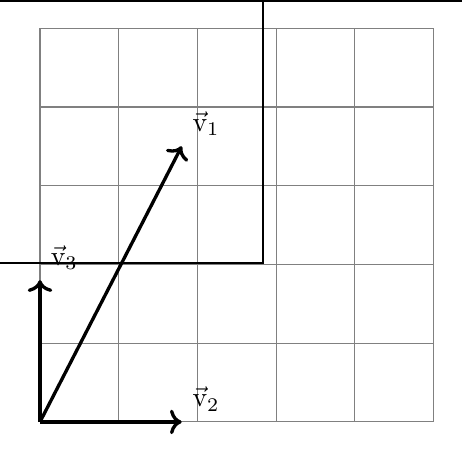
\begin{tikzpicture}
        \tkzInit[xmax=0.5,ymax=0.5,xstep=0.1,ystep=0.1]
        %\tkzAxeX[label=FancyBrand,above left=10pt]
        \tkzAxeX[label=FancyBrand, right]
        %\tkzAxeY[label=green,below right=30pt]
        \tkzAxeY[label=green,above]
        \tkzGrid
        \draw[very thick, ->] (0,0) -- (1.8,3.5) node[anchor=south west]{$\vec{\text{v}}_1$};
        \draw[very thick,latex-latex, ->] (0,0) -- (1.8,0) node[anchor=south west]{$\vec{\text{v}}_2$};
        \draw[very thick,latex-latex, ->] (0,0) -- (0, 1.8) node[anchor=south west]{$\vec{\text{v}}_3$};
    \end{tikzpicture}

    \caption{Two dimensional vector space model}
    \label{fig:vectorspacemodel}
\end{figure}




% evtl. noch ausf\"uhren:
% - stop words (woerter die nicht gewertet werden z.b. ist, er war, ...)
% - Parametric and zones indixes


\section{recommender algorithm}


\subsection{Information retrieval}
%%%%%%%%%%%%%%%%%%%%%%%%%%%%%%%%%
\iffalse
Was ist Information retrieval
in depth implementation is out of scope
Hinleitung zu Vektoren
\fi
%%%%%%%%%%%%%%%%%%%%%%%%%%%%%%%%%
\citeauthor{manning:2009} describe Information Retrieval in their book as process of "finding material [\dots] of an unstructured nature [\dots] that satisfies an information need from within a large collection."\citep[p.~1]{manning:2009}\\
In generall IR and RS are very similiar and a few technologies and findings of IR can be transfered to RS.
Since IR systems are build to handle unstructured data and transform them into a form that is easier to handle for computer systems one can adopt the method to RS input data such as items.\citep[p.~21-23]{ricci:2011}
There are various ways IR systems interpret data.
However this thesis will focus on one common method (and the theorie it depends on) called "tf-idf-vectors" which is a requirement for the Rocchio algorithm.\citep[p.~93]{lops:2011}\\
IR systems are built to handle "unstructured data".
Unstructured data is information bundled within a document (document is the IR related term for what is understood as item by RS) without any clear semantical structure.\citep[p.~1-3]{manning:2009}
The data within a document
IR systems can extract all relevant terms from a document
A term may resemble an attribute of an item such as its colour or brand.
The way of retrieving terms from a unstructured document is out of scope for this thesis but there is a brief example in figure~\ref{fig:TermRetrieving}.\\
For the section Information Retrieval the IR vocabulary will be adopted.
This means, that items will be called documents and attributes will be known as terms.

\begin{figure}[h]
    \center
    %\lstset{style=customHTML}
    \begin{lstlisting}
<html>
    <head><title>Online shop</title></head>
    <body>
        <img src="/img/p_42.jpg" alt="FancyBrand's product"/>
        <table>
            <tr><td>Colour</td><td>green</td></tr>
            <tr><td>Price</td><td>24,95 &euro;</td></tr>
            <tr><td>Brand</td><td>FancyBrand</td></tr>
        </table>
    </body>
</html>
    \end{lstlisting}
    \rowcolors{1}{\dustRowFirst}{\dustRowSecond}
    \begin{tabular}{ l }
        \rowcolor{\dustRowHead}
        \textbf{Terms:}\\\hline
        green\\
        24,95 \&euro;\\
        FancyBrand%\\\hline
    \end{tabular}
    \caption{Retrieving Terms from a HTML document.}
    \label{fig:TermRetrieving}
\end{figure}


\subsection{Weighting}
\label{sec:weighting}
As already mentioned a document can be be described as a collection of terms.
The process of locating terms within a document is taken for granted.
When a user queries for a specific term one has to find each relevant document including this term.
Also an order regarding the documents significance will be required.
The terms significance within a document is defined by its weight.\citep[p.~117]{manning:2009}\\
While primitive IR methods such as boolean retrieval only check for the existance of a queried term within a document weighting can give more precise results regarding the terms significance in a document.\citep[p.~109]{manning:2009}

\paragraph{Term frequency}
\label{sec:tf}
\index{Term Frequency}
A simple method to quantify the importance of a term within a document is the so called term frequency.
The concept is based on the assumption that the frequency of a term $t$ indicates its importance within a document $d$.
It is denoted as $\text{tf}_{t,d}$ where $t$ resembles the term an $d$ the document.
The number of occurences of $t$ within $d$ can be directly interpreted its term frequency.\citep[p.~117]{manning:2009}\\
For products of an online shop and its resulting term frequency may look like as described in figure~\ref{fig:tfweighting}.\\
\begin{figure}[h]

    \begin{quote}
        Document $\text{d}1$ with identified terms underlined:\\
        \underline{blouse} \underline{blue} \underline{55} Euro. \underline{55} cm by size \underline{S}. 100\% \underline{Polyester}
    \end{quote}

    \center
    \vspace{5mm}
    \rowcolors{0}{\dustRowFirst}{\dustRowSecond}
    \begin{tabular}{ l l }
        \rowcolor{\dustRowHead}
        \multicolumn{2}{c}{Term frequency}\\\hline
        $\text{tf}_{\text{blouse},\text{d1}}$       & 1\\
        $\text{tf}_{\text{blue},\text{d1}}$         & 1\\
        $\text{tf}_{\text{55},\text{d1}}$           & 2\\
        $\text{tf}_{\text{S},\text{d1}}$            & 1\\
        $\text{tf}_{\text{Polyester},\text{d1}}$    & 1\\
    \end{tabular}

    \caption{Term frequency weighting}
    \label{fig:tfweighting}
\end{figure}

\paragraph{Inverse document frequency}
\label{sec:idf}
\index{Inverse Document Frequency}
In some domains special terms will often appear multiple times within a document and therefore have high term frequency weight without giving any explanatory value.\citep[p.~117]{manning:2009}
Documents resembling clothing offered by an online shop may always include the name of the store as term.
Since the user already explicitely searches on the store, the relevance of this term is rather low.
In order to transfer this to weighting, inverse document weighting (idf) has been implemented.
Idf will scale down the weighting of terms that appear in all documents.
To do so, an intermediate step is neccessary. Before calculating the idf for a term one has to determine both the terms document frequency ($\text{df}_t$) and the total count of documents (as $N$).
Next the idf can be calculated with following forumla:\citep[p.~117-118]{manning:2009}\\
\begin{equation}
    \text{idf}_{t} = \log\frac{N}{\text{df}_{t}}
    \label{eq:idf-forumula}
\end{equation}
The logarithms basis isn't of great importance.\citep[p.~118]{manning:2009}
The examples however use 10 as base.
A more explanatory example is presented by figure~\ref{fig:idfweighting}.
The example states that rare items posses a higher idf, whereas more frequent terms are rated lower.\citep[p.~118]{manning:2009}\\
\begin{figure}[h]
    \begin{quote}
        Total count of documents  $N$ is 500\\
        Term1 "FancyShop" appears in 500 documents\\
        Term2 "blouse" appears in 130 documents\\
    \end{quote}

    \center
    \begin{tabular}{ l | l }
        $\text{df}_{\text{FancyShop}} = 500$                                                                    & $\text{df}_{\text{blouse}} = 130$\\
        $\text{idf}_{\text{FancyShop}} = \log\frac{N}{\text{df}_{\text{FancyShop}}} = \log\frac{500}{500} = 0$  & $\text{idf}_{\text{blouse}} = \log\frac{N}{\text{df}_{\text{blouse}}} = \log\frac{500}{130} \approx 0.59$
    \end{tabular}

    \caption{Inverse document frequency weighting}
    \label{fig:idfweighting}
\end{figure}

\paragraph{Tf-Idf}
\label{sec:tfidf}
\index{TfIdf}
Both the term frequency, as well as the inverse document frequency have some drawbacks.
While term frequency may weight terms with little informative value high because they appear often, inverse document frequency can totally ignore them by weighting them extremely low.
But it's possible to combine td and idf in order to get better weightings.
The result is called tf-idf.\citep[p.~118-119]{manning:2009}
\begin{equation}
    \text{tf-idf}_{\text{t,d}} = \text{tf}_\text{t,d} \times \text{idf}_\text{d}
    \label{eq:tf-idf-forumula}
\end{equation}

\noindent
Figure~\ref{fig:tfidfweighting} illustrates the generation of an tf-idf weighting.
\begin{figure}[h]

    \begin{quote}
        Total number of documents $N$ is 3\\
    \end{quote}

    \center
    \rowcolors{1}{\dustRowFirst}{\dustRowSecond}
    \begin{tabular}{ l l | l l l l }
        \rowcolor{\dustRowHead}
        Term                    & Document          & tf    & df & idf   & tf-idf\\\hline
        blouse                  & $\text{doc}_1$    & 15    &  2 & 0.18  & 2.7\\
        blouse                  & $\text{doc}_2$    & 5     &  2 & 0.18  & 0.9\\
        blouse                  & $\text{doc}_3$    & 9     &  2 & 0.18  & 1.62\\
    \end{tabular}
    \caption{tf-idf weighting}
    \label{fig:tfidfweighting}
\end{figure}

\noindent
\citeauthor{manning:2009} describes tf-idf weighting as follows:\\
"$\text{[Tf-idf}_{\text{t,d}}\text{]}$ assigns to term $t$ a weight in document $d$ that is
\begin{enumerate}
    \item highest when $t$ occurs many times within a small number of documents
    (thus lending high discriminating power to those documents);
    \item lower when the term occurs fewer times in a document, or occurs in many
    documents (thus offering a less pronounced relevance signal);
    \item lowest when the term occurs in virtually all documents."
\end{enumerate}
\citep[p.~119]{manning:2009}

\subsubsection{Vector space model}
\label{sec:vectorspacemodel}
\index{VectorSpaceModel}
Any document can now be described as a vector.
Each term in a document will be directly interpreted as component of a vector.
If a term is non existent in a document, the vector component will be numeric zero.\citep[p.~120]{manning:2009}\\
Therefore IR provids methods to describe documents as vectors.
Forging a bridge back to RS the vectors can help to provide a computer representation of real world products.
The vectors of all products can be displayed in one common vector space.
This process is known as vector space model.\citep[p.~120]{manning:2009}
An example of a two dimensional vector space model is given in figure~\ref{fig:vectorspacemodel}.


\begin{figure}[h]

    \begin{quote}
        There are three documents with following terms:\\
        Document $\text{d}_1$: $1\times \text{FancyBrand}, 2\times \text{green}$\\
        Document $\text{d}_2$: $1\times \text{FancyBrand}$\\
        Document $\text{d}_3$: $1\times \text{green}$\\
        Whereas "FancyBrand" and "green" are the document terms.

        \noindent
        The generic tf-idf vector representation of one of the documents above will be:\\
        $\vec{\text{v}}_{\text{generic}} = (\text{tf-idf}_{\text{FancyBrand},\text{d}_\text{generic}}, \text{tf-idf}_{\text{green},\text{d}_\text{generic}})^T$

        \noindent
        The corresponding tf-idf-vectors of the are:\\
        $\vec{\text{v}}_1 = (\text{tf-idf}_{\text{FancyBrand},\text{d}_1}, \text{tf-idf}_{\text{green},\text{d}_1})^T = (0.18, 0.35)^T$\\
        $\vec{\text{v}}_2 = (\text{tf-idf}_{\text{FancyBrand},\text{d}_2}, \text{tf-idf}_{\text{green},\text{d}_2})^T = (0.18, 0)^T$\\
        $\vec{\text{v}}_3 = (\text{tf-idf}_{\text{FancyBrand},\text{d}_3}, \text{tf-idf}_{\text{green},\text{d}_3})^T = (0, 0.18)^T$\\
    \end{quote}

    \center
    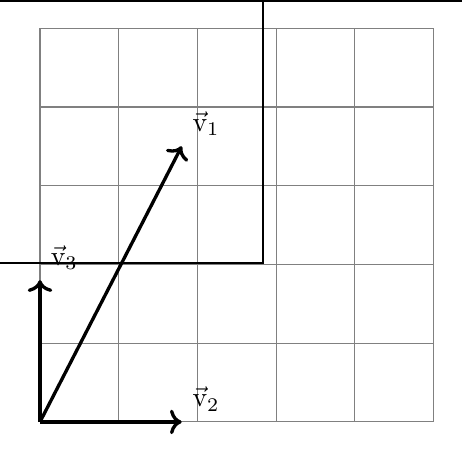
\begin{tikzpicture}
        \tkzInit[xmax=0.5,ymax=0.5,xstep=0.1,ystep=0.1]
        %\tkzAxeX[label=FancyBrand,above left=10pt]
        \tkzAxeX[label=FancyBrand, right]
        %\tkzAxeY[label=green,below right=30pt]
        \tkzAxeY[label=green,above]
        \tkzGrid
        \draw[very thick, ->] (0,0) -- (1.8,3.5) node[anchor=south west]{$\vec{\text{v}}_1$};
        \draw[very thick,latex-latex, ->] (0,0) -- (1.8,0) node[anchor=south west]{$\vec{\text{v}}_2$};
        \draw[very thick,latex-latex, ->] (0,0) -- (0, 1.8) node[anchor=south west]{$\vec{\text{v}}_3$};
    \end{tikzpicture}

    \caption{Two dimensional vector space model}
    \label{fig:vectorspacemodel}
\end{figure}


\subsubsection{Parametric and zone indices}
\label{sec:parametricandzoneindices}

% evtl. noch ausf\"uhren:
% - stop words (woerter die nicht gewertet werden z.b. ist, er war, ...)
% - Parametric and zones indices


\subsection{Rocchio's algorithm}
\label{sec:rocchio}
%%%%%%%%%%%%%%%%%%%%%%%%%%%%%%%%%%%%
\iffalse
Beschreibung des Rocchio algorithmus
\fi
%%%%%%%%%%%%%%%%%%%%%%%%%%%%%%%%%%%%
With section~\ref{sec:tfidf} and section~\ref{sec:vectorspacemodel} the requirements of Rocchio's algorithm have been described.\citep[p.~178]{manning:2009}
The next step is to specify the algorithm itself.
{\color{red} Kommt eigentlich aus information retrieval und hilft dabei items zu finden.
Bietet also vorschlaege zu einer suchanfrage, wobei die anfrage die bisher gewaehlten producte sind.}
Rocchio's relevance feedback algorithm is classified as content-based RS.\citep[p.~92]{lops:2011}
The algorithm tries to find a vector representing the user that is similiar to all item which are relevant to the user.
In addition the number of unrelevant item matching the vector should be minimal.\citep[p.~178-181]{manning:2009}
One of the algorithms charakteristics is the way feedback (as described in section~\ref{sec:feedback}) is treated.
Every time the user gives either positive or negative feedback, the algorithm will adapt the user vector to match the new criteria.\citep[p.~387-388]{pazzani:2007}
\\

When using Rocchio's algorithm for a recommender system one uses a user vector instead of a query vector as originally intended.
\begin{equation}
    \vec{\text{q}}_m =
        \alpha \cdot \vec{\text{q}}_0
        + \beta \cdot \frac{1}{|\text{D}_\text{r}|}\sum_{\vec{\text{d}}_j\in \text{D}_\text{r}} \vec{\text{d}}_j
        - \gamma \cdot \frac{1}{|\text{D}_\text{nr}|}\sum_{\vec{\text{d}}_j\in \text{D}_\text{nr}} \vec{\text{d}}_j
\end{equation}
$\vec{\text{q}}_0$ is the old vector representing the user before he gave feedback about one of the items.
The result $\vec{\text{q}}_m$ however is the modified vector describing the user after his most recent feedback has been considered.
For each calculation with Rocchio's algorithm $\vec{\text{q}}_0$ will always be the result $\vec{\text{q}}_m$ of the preceding calculation.\\
$\text{D}_\text{r}$ is a set of all relevant item vectors, while $\text{D}_\text{nr}$ represents a set of items that are unrelevant to the user.\\
$\alpha$, $\beta$ and $\gamma$ act as weights and can influence the importance of the old user vector, as well as of  the relevant and unrelevant documents.
The old user vector is weighted by $\alpha$.
The average of relevant documents is weighted by $\beta$ and $\gamma$ is responsible for unrelevant documents.
There are only positive values for weights allowed.
The lowest possible weight is 0.
A well established configuration for these weights is: $\alpha = 1$, $\beta = 0.75$ and $\gamma = 0.15$.
However if a RS only allows positive feedback, one can as well set $\gamma$ to 0.
\citep[p.~178-183]{manning:2009}



\section{Implementation}
Most of the theorie behind RS and the methodology it depends on have already been introduced.
The implementation of a RS will be described in the following.
The examples will be written in a programming language called Python.
There is also some SQL code and some UML- and EER-diagrams in order to visualize the concept.

\subsection{Content based RS in-depth}
\label{sec:implementation-contentbased}
The general framework for a content-based RS is shown in figure~\ref{fig:framework-contentbasedrs}.
There are three main components a content-based RS needs.
\begin{itemize}
    \item \textbf{Content Analyzer}\\
        Since all items the RS has to work with can potentially be unstructured, a pre-process is necessary to filter relevant information.
        This will be mainly done by techniques of IR.
        The Content Analyzer aims to bring all items in a from that can be used by its successional components.
        \citep[p.~75-77]{lops:2011}
    \item \textbf{Profile Learner}\\
        When the items are in a suitable form, the Profile Learner can construct a user profile.
        In case of Rocchio's algorithm this includes to distinguish all relevant items from non-relevant.
        With the items and the users preferences the Profile Learner can build the user profile.
        In case of Rocchio, the user profile is a vector representing his attitude towards the different attributes a item may have.
        \citep[p.~75-77]{lops:2011}
    \item \textbf{Filtering Component}\\
        For each user profile the Filtering Component can find items that may match the users preferences.
        Depending on the method implemented the result can be a binary or continuous relevance judgment.
        The continuous relevance judgement is a list of ranked items.
        \citep[p.~75-77]{lops:2011}
        The RS implemented for this thesis uses the k-nearest-neighbours (kNN) classification.
        This results in a list of ranked items where the $k$ best-ranked items will be suggested to the user.
\end{itemize}


\begin{figure}[h]
    \center
    \includegraphics[scale=0.3]{inc/implementation/HighlevelContentBased}
    \caption{High level description of a content-based RS.\citep[p.~76]{lops:2011}}
    \label{fig:framework-contentbasedrs}
\end{figure}



\subsection{Content Analyzer}
\label{sec:content-analyzer}
\index{Content Analyzer}
For this project the data describing the products, offered by an online shop have been semi-structured.
It was a text file where each line described a product.
An example is given in listing~\ref{lst:product-data}.

\begin{lstlisting}[caption={Example product data},label={lst:product-data}
    ,keywordstyle=\color{black}
    ,commentstyle=\itshape\color{black}
    ,identifierstyle=\color{black}
    ,stringstyle=\color{black}
]
ImgURL Brand Product Price Shoulder_Width Model_Length Collar_Type Material
http://i1.ztat.net/large/4E/M2/1E/00/0K/11/4EM21E000-K11@4.jpg Emoi en Plus Bluse - dazzling blue 24,95 °(\euro{})° 50 cm 70 cm bei Gr°(\"{o}\ss{})°e 44 Rundhals 100% Polyester
http://i2.ztat.net/large/NA/52/1D/03/NA/11/NA521D03N-A11@3.jpg NAF NAF WENT - Bluse - ecru/noir 38,95 °(\euro{})° 55 cm bei Gr°(\"o{}\ss{})°e S Rundhals 64% Viskose, 22% Baumwolle, 10% Modal, 4% Polyamid
\end{lstlisting}

%\noindent
%Since the structure of the input was known, it was possible to filter out all relevant product information without using too fancy IR methods.
%With regular expressions all relevant informations such as the product\_image-url, brand, product, price, collar type and material have been extracted and stored in a database.
From each line describing a product information such as the image URL and materials have been extracted.
Except from the image URL every word separated by whitespace has been interpreted as term.
Since a RS could theoretically handle any kind of item afar from products, a distinction has been made between documents in general and products.
The relation between a product and a document has been illustrated in figure~\ref{fig:ertermdocumentassignment}.
\begin{figure}[h]
    \center
    \includegraphics[scale=0.5]{inc/implementation/contentanalyzer/er_term_document_assignment}
    \caption{ER diagram of documents, products and associated terms}
    \label{fig:ertermdocumentassignment}
\end{figure}
Since the relation between \textit{Product} and \textit{Term} is N to N, an intermediate table is necessary when transforming the ER-diagram into a relational model.
Therefore the table \textit{TermDocumentAssigner} has been introduced and the relational model will look as follows:

\begin{quote}
    \textbf{Document}{(\underline{document\_id})}\\
    \textbf{Product}{(\underline{document\_id[Document]}, image\_name)}\\
    \textbf{Term}{(\underline{term\_id}, name)}\\
    \textbf{TermDocumentAssigner}{(\underline{document\_id[Document], term\_id[Term]}, count)}\\
\end{quote}

Because \textit{TermDocumentAssigner} will be very often used to query all terms of a document, it might be useful to create an index on \textit{document\_id}.
Implicitly there will also be one on the combined primary key \textit{document\_id, term\_id}.
The tables, implemented by the RS built for this thesis, filled with example data may look as in table~\ref{tab:tablestermdocumentproduct}.
Table~\ref{tab:tablestermdocumentproduct} will serve as resource for terms and documents to illustrate subsequent examples.

\begin{table}

    \center

    % Document
    \rowcolors{1}{\dustRowFirst}{\dustRowSecond}
    \begin{tabular}{ l }
        \rowcolor{\dustRowHead}
        \textbf{Document}\\\hline
        document\_id\\\hline
        1\\
        2\\
        3\\
    \end{tabular}
    \quad
    % Product
    \rowcolors{1}{\dustRowFirst}{\dustRowSecond}
    \begin{tabular}{ l | l }
        \rowcolor{\dustRowHead}
        \multicolumn{2}{ c }{\textbf{Product}}\\\hline
        document\_id    & image\_name\\\hline
        1               & image\_1.png\\
        2               & image\_2.png\\
        3               & image\_3.png\\
    \end{tabular}

    %~\\
    \hfill\\

    %TermDocumentAssigner
    \rowcolors{1}{\dustRowFirst}{\dustRowSecond}
    \begin{tabular}{ l | l | l }
        \rowcolor{\dustRowHead}
        \multicolumn{3}{c}{\textbf{TermDocumentAssigner}}\\\hline
        document\_id    & term\_id  & count\\\hline
        1               & 1         & 1\\
        1               & 2         & 1\\
        1               & 4         & 1\\
        2               & 1         & 1\\
        2               & 3         & 1\\
        2               & 7         & 1\\
        3               & 4         & 1\\
        3               & 5         & 1\\
        3               & 6         & 1\\
    \end{tabular}
    \quad
    % Term
    \rowcolors{1}{\dustRowFirst}{\dustRowSecond}
    \begin{tabular}{ l | l }
        \rowcolor{\dustRowHead}
        \multicolumn{2}{ c }{\textbf{Term}}\\\hline
        term\_id        & name\\\hline
        1               & blouse\\
        2               & blue\\
        3               & polyester\\
        4               & cotton\\
        5               & green\\
        6               & trouser\\
        7               & white\\
    \end{tabular}
    \caption{Table layout defined by figure~\ref{fig:ertermdocumentassignment}}
    \label{tab:tablestermdocumentproduct}
\end{table}

%\noindent
As already mentioned before, Rocchio's algorithm works best with tf-idf vectors.
With the theory described in section~\ref{sec:tfidf} the next big step is to show how vectors for this project have been built.
As a short reminder: all products are described through their terms.

In order to build tf-idf vectors, one also has to build term frequency-, as well as inverse document frequency vectors - these are the preconditions.
Since these tasks are fairly similar, some design patterns help realizing them.
The \gls{abstract factory} pattern proofed to be very handy for this task.
For each necessary vector (tf, idf, tf-idf) one can build a vector creator which shares the design of the other vector creators.
Therefore the abstract class \textit{VectorCreator} has been introduced.
The \textit{VectorCreator} offers the abstract method \textit{\_get\_vector(document\_id:int):DocumentVector} which will be responsible for creating all vectors.
All inherited classes will implement the abstract method with a procedure to create an instance of \textit{DocumentVector}.

\FloatBarrier

\paragraph{Term frequency vector}
\index{Term Frequency}
A term frequency vector representing a document consists of the count of a term's occurrences.
The current implementation uses the SQL query displayed in listing~\ref{lst:tf-query} for generating the tf vector.
The result of a query may look as follows (based on the tables shown in figure~\ref{fig:ertermdocumentassignment} and are displayed in table~\ref{tab:tf-query-result}.

\begin{table}

    \center

    \rowcolors{1}{\dustRowFirst}{\dustRowSecond}
    \begin{tabular}{ l|l|l }
        \rowcolor{\dustRowHead}
        \multicolumn{3}{c}{\textbf{$\text{tf}_\text{document\_1}$}}\\\hline

        term\_id & name & value \\\hline
        1   & blouse    & 1\\
        2   & blue      & 1\\
        3   & polyester & 0\\
        4   & cotton    & 1\\
        5   & green     & 0\\
        6   & trouser   & 0\\
        7   & white     & 0\\
    \end{tabular}
    \quad
    \rowcolors{1}{\dustRowFirst}{\dustRowSecond}
    \begin{tabular}{ l|l|l }
        \rowcolor{\dustRowHead}

        \multicolumn{3}{c}{\textbf{$\text{tf}_\text{document\_2}$}}\\\hline

        term\_id & name  & value\\\hline
        1    & blouse    & 1\\
        2    & blue      & 0\\
        3    & polyester & 1\\
        4    & cotton    & 0\\
        5    & green     & 0\\
        6    & trouser   & 0\\
        7    & white     & 1\\
    \end{tabular}
    \hfill\\
    \rowcolors{1}{\dustRowFirst}{\dustRowSecond}
    \begin{tabular}{ l|l|l }
        \rowcolor{\dustRowHead}
        \multicolumn{3}{ c }{\textbf{$\text{tf}_\text{document\_3}$}}\\\hline

        term\_id & name & value\\\hline
        1 & blouse  & 0\\
        2 & blue  & 0\\
        3 & polyester  & 0\\
        4 & cotton  & 1\\
        5 & green  & 1\\
        6 & trouser  & 1\\
        7 & white  & 0\\
    \end{tabular}

    \caption{Possible result of the query in listing~\ref{lst:tf-query}}
    \label{tab:tf-query-result}
\end{table}

\begin{lstlisting}[language=SQL,caption={SQL query for generating tf-vectors},label={lst:tf-query},float=h]
-- :document_id is a parameter given to the method
SELECT
    [t].[term_id]
    , [t].[name]
    , CASE WHEN  [a].[document_id] IS NULL
        THEN    0
        ELSE    [a].[count]
    END AS [value]
FROM
    [Term] AS [t]
    LEFT OUTER JOIN [TermDocumentAssigner] AS [a]
        ON  [t].[term_id] = [a].[term_id]
        AND [document_id] = :document_id
ORDER BY
    [t].[term_id]
;
\end{lstlisting}

The result of the query shown in listing~\ref{lst:tf-query} will finally be stored in the \textit{TermFrequencyVector} class derived from \textit{DocumentVector} (see figure~\ref{fig:uml-document-vectors}).

\FloatBarrier

\paragraph{Document frequency vector}
\index{Document Frequency}
In contrast to \textit{TermFrequencyVector} the \textit{DocumentFrequencyVector} resembles the whole collection of documents, rather than a single one.
Therefore the parameter \textit{document\_id} can be omitted.
But in order to sustain uniformity between all classes inheriting from \textit{VectorCreator} it will be carried along but set to a null value.
To make the source code more readable, the SQL code for querying the document-frequency values has been outsourced to a SQL-View as shown in listing~\ref{lst:df-view}.
This little tweak (which has no influence on execution-speed) left the query for df-vectors as simple as shown in listing~\ref{lst:df-query}.
The result for the example is given in table~\ref{tab:df-query-result}.

\begin{lstlisting}[language=SQL,caption={SQL statement to create the \textit{DocumentFrequency}-view},label={lst:df-view},float=h]
CREATE VIEW IF NOT EXISTS [DocumentFrequency] AS
    SELECT
            [t].[term_id]
            , [t].[name]
            , CASE WHEN   [a].[count] IS NULL
                THEN        0
                ELSE        [a].[count]
            END AS [value]
    FROM
        [Term] as [t]
        LEFT OUTER JOIN
        (
            SELECT
                [term_id]
                , SUM([document_id]) AS [count]
            FROM
                [TermDocumentAssigner]
            GROUP BY
                [term_id]
        ) AS [a]
            ON [t].[term_id] = [a].[term_id]
    ORDER BY
        [t].[term_id]
;
\end{lstlisting}

\begin{lstlisting}[language=SQL,caption={SQL query for generating df-vectors},label={lst:df-query},float=h]
SELECT
    [term_id]
    , [name]
    , [value]
FROM
    [DocumentFrequency]
;
\end{lstlisting}

\begin{table}
    \center
    \rowcolors{1}{\dustRowFirst}{\dustRowSecond}
    \begin{tabular}{ l | l | l }
        \rowcolor{\dustRowHead}
        \multicolumn{3}{ c }{\textbf{df}}\\\hline
        term\_id    & name      & value\\\hline
        1           & blouse    & 2\\
        2           & blue      & 1\\
        3           & polyester & 1\\
        4           & cotton    & 2\\
        5           & green     & 1\\
        6           & trouser   & 1\\
        7           & white     & 1\\
    \end{tabular}
    \caption{Possible results of the query in figure~\ref{lst:df-query}}
    \label{tab:df-query-result}
\end{table}

\begin{figure}[h]
    \center
    \includegraphics[scale=0.4]{inc/implementation/contentanalyzer/uml_document_vectors}
    \caption{Document vectors}
    \label{fig:uml-document-vectors}
\end{figure}

\FloatBarrier

\paragraph{Inverse document frequency vector}
\index{Inverse Document Frequency}
For building idf-vectors one can use df-vectors (and their source code) as basis.
The inverse document frequency is the logarithm of the total count of documents in a collection divided by a term's document frequency.
Another SQL-View called N-view will provide the number of documents, while the code for creating idf-vectors get outsourced into its own view once more.
Since the SQL implementation of \gls{sqlite3} does not offer a logarithm-function, one has to define his very own.
Fortunately the standard python library for connecting to sqlite3-databases supports the creation of functions as shown in listing~\ref{lst:idf-log-function}.


\begin{lstlisting}[language=Python,caption={Preparing the log-function for SQL-statement in listing~\ref{lst:idf-view}},label={lst:idf-log-function},float=h]
def _create_log_function(self, conn):
    conn.create_function('log10', 1, InverseDocumentFrequencyVectorCreator.log_10)
    pass

def log_10(x):
    base = 10
    return math.log(x, base)
\end{lstlisting}
\begin{lstlisting}[language=SQL,caption={SQL-statement to create the InverseDocumentFrequency-view},label{lst:idf-view},float=h]
CREATE VIEW IF NOT EXISTS [InverseDocumentFrequency] AS
    SELECT
        [term_id]
        , [name]
        , log10
        (
            CAST ((SELECT [document_count] from [N]) AS REAL) / [df].[value]
        )
         AS [value]
    FROM
        [DocumentFrequency] AS [df]
    ORDER BY
        [term_id]
    ;
\end{lstlisting}


\begin{lstlisting}[language=SQL,caption={SQL-statement to create the N-view},label={lst:n-view},float=h]
CREATE VIEW IF NOT EXISTS [N] AS
    SELECT
        (SELECT COUNT(*) FROM [Document]) AS [document_count]
        , (SELECT COUNT(*) FROM [Term]) AS [term_count]
;
\end{lstlisting}


\begin{lstlisting}[language=SQL,caption={SQL-query for generating idf-vectors},label={fig:idf-query},float=h]
SELECT
    [term_id]
    , [name]
    , [value]
FROM
    [InverseDocumentFrequency]
;
\end{lstlisting}


\begin{table}
    \center
    \rowcolors{1}{\dustRowFirst}{\dustRowSecond}
    \begin{tabular}{ l | l | l }
        \rowcolor{\dustRowHead}
        \multicolumn{3}{ c }{\textbf{idf}}\\\hline
        term\_id    & name      & value\\\hline
        1           & blouse    & $\log_{10}(3/2) \approx 0.18$\\
        2           & blue      & $\log_{10}(3/1) \approx 0.48$\\
        3           & polyester & $\log_{10}(3/1) \approx 0.48$\\
        4           & cotton    & $\log_{10}(3/2) \approx 0.18$\\
        5           & green     & $\log_{10}(3/1) \approx 0.48$\\
        6           & trouser   & $\log_{10}(3/1) \approx 0.48$\\
        7           & white     & $\log_{10}(3/1) \approx 0.48$\\
    \end{tabular}
    \caption{Possible results of the query in figure~\ref{fig:idf-query}}
    \label{tab:idf-query-result}
\end{table}

\FloatBarrier

\paragraph{Tf-idf vector}
\index{TfIdf}
Finally one can create tf-idf vectors which are the combination of tf- and idf-vectors (as explained in section~\ref{sec:tfidf}).
Since tf-idf is merely the multiplication of term frequency with the corresponding inverse document frequency, it is rather simple to create.
Listing~\ref{lst:tfidf-code} shows the creation of a \textit{TfIdfVector} in the method \textit{\_create\_vector()}, whereas the multiplication is in method \textit{\_get\_values()}.

\begin{lstlisting}[language=Python,caption={Python code for calculating tfidf-vectos on basis on tf- and idf-vectors},label={lst:tfidf-code},float=h]
class TfIdfVectorCreator(VectorCreator):

    def __init__(self, db_connection_str):
        super(TfIdfVectorCreator, self).__init__(db_connection_str)

        self._tf_creator = TermFrequencyVectorCreator(db_connection_str)
        self._idf_creator = InverseDocumentFrequencyVectorCreator(db_connection_str)
        pass

    def _create_vector(self, document_id):
        tf_vector = self._tf_creator.get_vector(document_id)
        idf_vector = self._idf_creator.get_vector(document_id)

        tfidf_vector = TfIdfVector()

        for triple in self._get_values(tf_vector, idf_vector):
            tfidf_vector.add_to_vector(triple)

        return tfidf_vector

    def _get_values(self, tfv, idfv):
        ingredients = zip(tfv.term_id, tfv.description, tfv.values, idfv.values)

        for (tf_tid, tf_desc, tf_val, idf_val) in ingredients:
            yield (tf_tid, tf_desc, tf_val * idf_val)
            pass
        pass
\end{lstlisting}

\begin{table}
    \center

    \rowcolors{1}{\dustRowFirst}{\dustRowSecond}
    \begin{tabular}{ l|l|l }
        \rowcolor{\dustRowHead}
        \multicolumn{3}{ c }{\textbf{$\text{tf-idf}_\text{document\_1}$}}\\\hline
        term\_id & name & value\\\hline
        1   & blouse    & $\approx 0.18$\\
        2   & blue      & $\approx 0.48$\\
        3   & polyester & 0\\
        4   & cotton    & $\approx 0.18$\\
        5   & green     & 0\\
        6   & trouser   & 0\\
        7   & white     & 0\\
    \end{tabular}
    \quad
    \rowcolors{1}{\dustRowFirst}{\dustRowSecond}
    \begin{tabular}{ l|l|l }
        \rowcolor{\dustRowHead}
        \multicolumn{3}{ c }{\textbf{$\text{tf-idf}_\text{document\_2}$}}\\\hline
        term\_id & name & value\\\hline
        1    & blouse   & $\approx 0.18$\\
        2    & blue     & 0\\
        3    & polyester& $\approx 0.48$\\
        4    & cotton   & 0\\
        5    & green    & 0\\
        6    & trouser  & 0\\
        7    & white    & $\approx 0.48$\\
    \end{tabular}

    \hfill\\

    \rowcolors{1}{\dustRowFirst}{\dustRowSecond}
    \begin{tabular}{ l|l|l }
        \rowcolor{\dustRowHead}
        \multicolumn{3}{ c }{\textbf{$\text{tf-idf}_\text{document\_3}$}}\\\hline

        term\_id & name & value\\\hline
        1        & blouse      & 0\\
        2        & blue        & 0\\
        3        & polyester   & 0\\
        4        & cotton      & $\approx 0.18$\\
        5        & green       & $\approx 0.48$\\
        6        & trouser     & $\approx 0.48$\\
        7        & white       & 0\\
    \end{tabular}


    \caption{Possible result of the function in figure~\ref{lst:tfidf-code}}
    \label{tab:tfidf-query-result}
\end{table}


With the vectors built, the main task of the content analyzer is done.
However there is still one more enhancement one can implement to make the repetitive creation of vectors faster.
Through \gls{dynamic programming} one can easily ``re-create" vectors which have already been used once.
Since it proves useful, if all inheriting classes of \textit{VectorCreator} can use dynamic programming without explicitly implementing it, one can implement the \textit{VectorCreator} as \gls{proxy}.
As a result the \textit{VectorCreator} gets another method called \textit{get\_vector(document\_id:int)} to which the same rules apply as to \textit{\_create\_vector(document\_id:int)}.
The buffering of \textit{DocumentVectors} can now be implemented in \textit{get\_vector(document\_id:int)} and all inheriting classes will also posses caching capabilities.
The code for dynamic programming is shown in listing~\ref{lst:dynamic-programming}.\\
In order to get a picture of all important vectors and their creation, a UML-diagram has been included (figure~\ref{fig:uml-vectorssimple}).

\begin{lstlisting}[language=Python,caption={Dynamic programming},label={lst:dynamic-programming},float=h]
class VectorCreator(object):

    # ... omitted unnecessary code

    def get_vector(self, document_id=None):
        if document_id is not None and not isinstance(document_id, int):
            raise TypeError('document_id must either be an integer or None')
        if not document_id in self._cache:
            vector = self._create_vector(document_id)
            if vector.document_id is None:
                vector.document_id = document_id
            self._cache[document_id] = vector
        return self._cache[document_id]}

    def _create_vector(self, document_id):
        # ... creating vector
\end{lstlisting}


\begin{figure}[h]
    \center
    \includegraphics[scale=0.33,angle=90]{inc/implementation/contentanalyzer/uml_vectors_simple}
    \caption{Abstract and concrete vector fabric}
    \label{fig:uml-vectorssimple}
\end{figure}

\FloatBarrier

\subsection{Profile Learner}
%{Rocchio algorithm}
%{Relevance feedback}


\FloatBarrier

\subsection{Filtering Component}
%%%%%%%%%%%%%%%%%%%%%%%%%%
%k nearest neighbours
% manning 297, 290 (euclidean distance)
%%%%%%%%%%%%%%%%%%%%%%%%%%

\FloatBarrier


\subsection{Online shop}
... dunno

\subsection{Testing and findings}
wie sind die Empfehlungen des algorithmus






\section{Technical details}

\subsection{Design patterns}

\subsubsection{Abstract factory}
\label{sec:abstractfactory}
\citeauthor{gamma:1993} describe a design pattern in their book "Design Patterns" that can be applied to this problem.
An abstract factory helps "creating families of related or dependent objects without specifying their concrete class"\citep[p.~99]{gamma:1993}.\\

\subsubsection{Proxy}
\label{sec:proxy}
% proxy page  233

\subsection{Dynamic programming}
\label{sec:dynamic-programmming}

\subsection{Python}

\subsection{Web API}

\subsection{node.js}

\subsection{git}





\section{Outlook}
%%%%%%%%%%%%%%%%%%%%%%%%%%%%%%
Was kann man noch alles mit recommender dingern machen?
- im physischem geschaeft
%%%%%%%%%%%%%%%%%%%%%%%%%%%%%%



% the license
%\input{inc/license/license}

% affidavit/sworn declaration



\section*{Eidesstattliche Erklärung}

 Ich erkläre hiermit an Eides Statt, dass ich die vorliegende Arbeit selbständig und ohne fremde Hilfe angefertigt und alle Abschnitte, die wörtlich oder annähernd wörtlich aus einer Veröffentlichung entnommen sind, als solche kenntlich gemacht habe, ferner, dass die Arbeit noch nicht veröffentlicht und auch keiner Prüfungsbehörde vorgelegt worden ist.

\bigskip
\noindent
 Fürth, den 24.12.0000


% print glossary
%\makeglossaries

% Abbildungsverzeichnis
\listoffigures

%bibliograpy
\bibliographystyle{abbrvnat}
\bibliography{thesis}

\end{document}
